\PassOptionsToPackage{unicode=true}{hyperref} % options for packages loaded elsewhere
\PassOptionsToPackage{hyphens}{url}
%
\documentclass[
]{article}
\usepackage{lmodern}
\usepackage{amssymb,amsmath}
\usepackage{ifxetex,ifluatex}
\ifnum 0\ifxetex 1\fi\ifluatex 1\fi=0 % if pdftex
  \usepackage[T1]{fontenc}
  \usepackage[utf8]{inputenc}
  \usepackage{textcomp} % provides euro and other symbols
\else % if luatex or xelatex
  \usepackage{unicode-math}
  \defaultfontfeatures{Scale=MatchLowercase}
  \defaultfontfeatures[\rmfamily]{Ligatures=TeX,Scale=1}
\fi
% use upquote if available, for straight quotes in verbatim environments
\IfFileExists{upquote.sty}{\usepackage{upquote}}{}
\IfFileExists{microtype.sty}{% use microtype if available
  \usepackage[]{microtype}
  \UseMicrotypeSet[protrusion]{basicmath} % disable protrusion for tt fonts
}{}
\makeatletter
\@ifundefined{KOMAClassName}{% if non-KOMA class
  \IfFileExists{parskip.sty}{%
    \usepackage{parskip}
  }{% else
    \setlength{\parindent}{0pt}
    \setlength{\parskip}{6pt plus 2pt minus 1pt}}
}{% if KOMA class
  \KOMAoptions{parskip=half}}
\makeatother
\usepackage{xcolor}
\IfFileExists{xurl.sty}{\usepackage{xurl}}{} % add URL line breaks if available
\IfFileExists{bookmark.sty}{\usepackage{bookmark}}{\usepackage{hyperref}}
\hypersetup{
  pdftitle={Spatial Autocorrelation \& Heteroscedasticity},
  pdfauthor={Yalin Yang},
  pdfborder={0 0 0},
  breaklinks=true}
\urlstyle{same}  % don't use monospace font for urls
\usepackage[margin=1in]{geometry}
\usepackage{color}
\usepackage{fancyvrb}
\newcommand{\VerbBar}{|}
\newcommand{\VERB}{\Verb[commandchars=\\\{\}]}
\DefineVerbatimEnvironment{Highlighting}{Verbatim}{commandchars=\\\{\}}
% Add ',fontsize=\small' for more characters per line
\usepackage{framed}
\definecolor{shadecolor}{RGB}{248,248,248}
\newenvironment{Shaded}{\begin{snugshade}}{\end{snugshade}}
\newcommand{\AlertTok}[1]{\textcolor[rgb]{0.94,0.16,0.16}{#1}}
\newcommand{\AnnotationTok}[1]{\textcolor[rgb]{0.56,0.35,0.01}{\textbf{\textit{#1}}}}
\newcommand{\AttributeTok}[1]{\textcolor[rgb]{0.77,0.63,0.00}{#1}}
\newcommand{\BaseNTok}[1]{\textcolor[rgb]{0.00,0.00,0.81}{#1}}
\newcommand{\BuiltInTok}[1]{#1}
\newcommand{\CharTok}[1]{\textcolor[rgb]{0.31,0.60,0.02}{#1}}
\newcommand{\CommentTok}[1]{\textcolor[rgb]{0.56,0.35,0.01}{\textit{#1}}}
\newcommand{\CommentVarTok}[1]{\textcolor[rgb]{0.56,0.35,0.01}{\textbf{\textit{#1}}}}
\newcommand{\ConstantTok}[1]{\textcolor[rgb]{0.00,0.00,0.00}{#1}}
\newcommand{\ControlFlowTok}[1]{\textcolor[rgb]{0.13,0.29,0.53}{\textbf{#1}}}
\newcommand{\DataTypeTok}[1]{\textcolor[rgb]{0.13,0.29,0.53}{#1}}
\newcommand{\DecValTok}[1]{\textcolor[rgb]{0.00,0.00,0.81}{#1}}
\newcommand{\DocumentationTok}[1]{\textcolor[rgb]{0.56,0.35,0.01}{\textbf{\textit{#1}}}}
\newcommand{\ErrorTok}[1]{\textcolor[rgb]{0.64,0.00,0.00}{\textbf{#1}}}
\newcommand{\ExtensionTok}[1]{#1}
\newcommand{\FloatTok}[1]{\textcolor[rgb]{0.00,0.00,0.81}{#1}}
\newcommand{\FunctionTok}[1]{\textcolor[rgb]{0.00,0.00,0.00}{#1}}
\newcommand{\ImportTok}[1]{#1}
\newcommand{\InformationTok}[1]{\textcolor[rgb]{0.56,0.35,0.01}{\textbf{\textit{#1}}}}
\newcommand{\KeywordTok}[1]{\textcolor[rgb]{0.13,0.29,0.53}{\textbf{#1}}}
\newcommand{\NormalTok}[1]{#1}
\newcommand{\OperatorTok}[1]{\textcolor[rgb]{0.81,0.36,0.00}{\textbf{#1}}}
\newcommand{\OtherTok}[1]{\textcolor[rgb]{0.56,0.35,0.01}{#1}}
\newcommand{\PreprocessorTok}[1]{\textcolor[rgb]{0.56,0.35,0.01}{\textit{#1}}}
\newcommand{\RegionMarkerTok}[1]{#1}
\newcommand{\SpecialCharTok}[1]{\textcolor[rgb]{0.00,0.00,0.00}{#1}}
\newcommand{\SpecialStringTok}[1]{\textcolor[rgb]{0.31,0.60,0.02}{#1}}
\newcommand{\StringTok}[1]{\textcolor[rgb]{0.31,0.60,0.02}{#1}}
\newcommand{\VariableTok}[1]{\textcolor[rgb]{0.00,0.00,0.00}{#1}}
\newcommand{\VerbatimStringTok}[1]{\textcolor[rgb]{0.31,0.60,0.02}{#1}}
\newcommand{\WarningTok}[1]{\textcolor[rgb]{0.56,0.35,0.01}{\textbf{\textit{#1}}}}
\usepackage{graphicx,grffile}
\makeatletter
\def\maxwidth{\ifdim\Gin@nat@width>\linewidth\linewidth\else\Gin@nat@width\fi}
\def\maxheight{\ifdim\Gin@nat@height>\textheight\textheight\else\Gin@nat@height\fi}
\makeatother
% Scale images if necessary, so that they will not overflow the page
% margins by default, and it is still possible to overwrite the defaults
% using explicit options in \includegraphics[width, height, ...]{}
\setkeys{Gin}{width=\maxwidth,height=\maxheight,keepaspectratio}
\setlength{\emergencystretch}{3em}  % prevent overfull lines
\providecommand{\tightlist}{%
  \setlength{\itemsep}{0pt}\setlength{\parskip}{0pt}}
\setcounter{secnumdepth}{-2}
% Redefines (sub)paragraphs to behave more like sections
\ifx\paragraph\undefined\else
  \let\oldparagraph\paragraph
  \renewcommand{\paragraph}[1]{\oldparagraph{#1}\mbox{}}
\fi
\ifx\subparagraph\undefined\else
  \let\oldsubparagraph\subparagraph
  \renewcommand{\subparagraph}[1]{\oldsubparagraph{#1}\mbox{}}
\fi

% set default figure placement to htbp
\makeatletter
\def\fps@figure{htbp}
\makeatother


\title{Spatial Autocorrelation \& Heteroscedasticity}
\author{Yalin Yang}
\date{2020-05-04}

\begin{document}
\maketitle

{
\setcounter{tocdepth}{3}
\tableofcontents
}
\hypertarget{maximum-likelihood}{%
\section{Maximum Likelihood}\label{maximum-likelihood}}

\hypertarget{evaluate-the-likelihood-and-log-likelhood-functions}{%
\subsection{Evaluate the likelihood and log-likelhood
functions}\label{evaluate-the-likelihood-and-log-likelhood-functions}}

The following code-chunks evaluate the likelihood function
\(L(\pi \mid x,n)=\pi^x \cdot (1-\pi)^{n-x}\) and the log-likelihood
function of a binary distributed outcomes \(x_i \in \{0,1\}\).

Set up the model:

\begin{Shaded}
\begin{Highlighting}[]
\OperatorTok{>}\StringTok{ }\NormalTok{pi <-}\StringTok{ }\DecValTok{1}\OperatorTok{:}\DecValTok{99}\OperatorTok{/}\DecValTok{100}                                 \CommentTok{# sequence of valid pi values}
\OperatorTok{>}\StringTok{ }\NormalTok{x <-}\StringTok{ }\DecValTok{7}                                         \CommentTok{# number of successes}
\OperatorTok{>}\StringTok{ }\NormalTok{n <-}\StringTok{ }\DecValTok{10}                                        \CommentTok{# number of trails}
\OperatorTok{>}\StringTok{ }\NormalTok{likFunc <-}\StringTok{ }\ControlFlowTok{function}\NormalTok{(x,n,pi) pi}\OperatorTok{^}\NormalTok{x}\OperatorTok{*}\NormalTok{(}\DecValTok{1}\OperatorTok{-}\NormalTok{pi)}\OperatorTok{^}\NormalTok{(n}\OperatorTok{-}\NormalTok{x)  }\CommentTok{# likelihood function}
\end{Highlighting}
\end{Shaded}

It shows, by example, that the maximum \(\pi_{max}\) of both functions
with the number of successes 7 and the number of trails 10 is the
\emph{identical}.

Plot the likelihood function \(L(\pi \mid x,n)\)

\begin{Shaded}
\begin{Highlighting}[]
\OperatorTok{>}\StringTok{ }\KeywordTok{plot}\NormalTok{(pi,}\KeywordTok{likFunc}\NormalTok{(x,n,pi), }\DataTypeTok{type=}\StringTok{"l"}\NormalTok{, }\DataTypeTok{xlab=}\KeywordTok{expression}\NormalTok{(pi), }
\OperatorTok{+}\StringTok{      }\DataTypeTok{ylab=}\StringTok{"likelihood function"}\NormalTok{)}
\OperatorTok{>}\StringTok{ }\KeywordTok{abline}\NormalTok{(}\DataTypeTok{v=}\NormalTok{x}\OperatorTok{/}\NormalTok{n, }\DataTypeTok{lty=}\DecValTok{5}\NormalTok{, }\DataTypeTok{col=}\StringTok{"red"}\NormalTok{)}
\end{Highlighting}
\end{Shaded}

\includegraphics{Lecture06_files/figure-latex/lik-1.pdf}

Plot the log-likelihood function \(\log(L(\pi \mid x,n))\)

\begin{Shaded}
\begin{Highlighting}[]
\OperatorTok{>}\StringTok{ }\KeywordTok{plot}\NormalTok{(pi,}\KeywordTok{log}\NormalTok{(}\KeywordTok{likFunc}\NormalTok{(x,n,pi)), }\DataTypeTok{type=}\StringTok{"l"}\NormalTok{, }\DataTypeTok{xlab=}\KeywordTok{expression}\NormalTok{(pi), }
\OperatorTok{+}\StringTok{      }\DataTypeTok{ylab=}\StringTok{"log-likelihood function"}\NormalTok{)}
\OperatorTok{>}\StringTok{ }\KeywordTok{abline}\NormalTok{(}\DataTypeTok{v=}\NormalTok{x}\OperatorTok{/}\NormalTok{n, }\DataTypeTok{lty=}\DecValTok{5}\NormalTok{, }\DataTypeTok{col=}\StringTok{"red"}\NormalTok{)}
\end{Highlighting}
\end{Shaded}

\includegraphics{Lecture06_files/figure-latex/loglik-1.pdf}

The numerical solution for \(\hat{\pi} = \frac{x}{n}\) The
log-likelihood function is: \[
\log(L(\pi)) \stackrel{\rm def}{=}
    \log(\pi^x \cdot (1-\pi)^{n-x}) = x \cdot \log \pi + (n-x) \cdot \log (1-\pi)  
\]

Its first derivative becomes: \[
\frac{d \log(L(\pi))}{d \pi}  =  \frac{x}{\pi} + \frac{n-x}{1-\pi} \cdot -1 =  \frac{x}{\pi} - \frac{n-x}{1-\pi}
\]

Setting the first derivative equal to zero gives the desired estimator
\hat{\pi} = \frac{x}{n}: \[
\frac{x}{\pi} - \frac{n-x}{1-\pi} = 0 \Rightarrow \hat{\pi} = \frac{x}{n}
\]

\hypertarget{heteroscedasticity}{%
\section{Heteroscedasticity}\label{heteroscedasticity}}

\hypertarget{read-data-explore-data}{%
\subsection{Read data \& explore data}\label{read-data-explore-data}}

\begin{Shaded}
\begin{Highlighting}[]
\OperatorTok{>}\StringTok{ }\KeywordTok{rm}\NormalTok{(}\DataTypeTok{list=}\KeywordTok{ls}\NormalTok{())}
\OperatorTok{>}\StringTok{ }\KeywordTok{library}\NormalTok{(TexMix)}
\OperatorTok{>}\StringTok{ }\KeywordTok{setwd}\NormalTok{(}\StringTok{"G:}\CharTok{\textbackslash{}\textbackslash{}}\StringTok{UTD_Classes}\CharTok{\textbackslash{}\textbackslash{}}\StringTok{2020Spring}\CharTok{\textbackslash{}\textbackslash{}}\StringTok{GISC7310_AdvancedDataAnalysis}\CharTok{\textbackslash{}\textbackslash{}}\StringTok{06Spatial Autocorrelation"}\NormalTok{)}
\OperatorTok{>}\StringTok{ }\NormalTok{Bladder <-}\StringTok{ }\NormalTok{foreign}\OperatorTok{::}\KeywordTok{read.spss}\NormalTok{(}\StringTok{"bladder_wmp2.sav"}\NormalTok{,}\DataTypeTok{to.data.frame=}\OtherTok{TRUE}\NormalTok{)}
\OperatorTok{>}\StringTok{ }
\ErrorTok{>}\StringTok{ }\NormalTok{car}\OperatorTok{::}\KeywordTok{scatterplotMatrix}\NormalTok{(}\OperatorTok{~}\NormalTok{bladp2}\OperatorTok{+}\NormalTok{lungp1}\OperatorTok{+}\NormalTok{popden, }\DataTypeTok{data=}\NormalTok{Bladder)}
\end{Highlighting}
\end{Shaded}

\includegraphics{Lecture06_files/figure-latex/unnamed-chunk-1-1.pdf}

\begin{Shaded}
\begin{Highlighting}[]
\OperatorTok{>}\StringTok{ }\NormalTok{car}\OperatorTok{::}\KeywordTok{scatterplotMatrix}\NormalTok{(}\OperatorTok{~}\KeywordTok{log}\NormalTok{(bladp2)}\OperatorTok{+}\KeywordTok{log}\NormalTok{(lungp1)}\OperatorTok{+}\KeywordTok{log}\NormalTok{(popden), }\DataTypeTok{data=}\NormalTok{Bladder)}
\end{Highlighting}
\end{Shaded}

\includegraphics{Lecture06_files/figure-latex/unnamed-chunk-1-2.pdf}

\begin{Shaded}
\begin{Highlighting}[]
\OperatorTok{>}\StringTok{ }\KeywordTok{hist}\NormalTok{(Bladder}\OperatorTok{$}\NormalTok{pop, }\DataTypeTok{breaks=}\DecValTok{20}\NormalTok{, }\DataTypeTok{freq=}\OtherTok{FALSE}\NormalTok{, }\DataTypeTok{xlab=}\StringTok{"Population at Risk"}\NormalTok{)}
\OperatorTok{>}\StringTok{ }\KeywordTok{lines}\NormalTok{(}\KeywordTok{density}\NormalTok{(Bladder}\OperatorTok{$}\NormalTok{pop), }\DataTypeTok{col=}\StringTok{"red"}\NormalTok{)}
\end{Highlighting}
\end{Shaded}

\includegraphics{Lecture06_files/figure-latex/unnamed-chunk-1-3.pdf}
Note: these data are \emph{areal aggregates} therefore there will be
some \emph{ecological biases} in the model estimates.

\hypertarget{variables-description}{%
\subsection{Variables description}\label{variables-description}}

\begin{itemize}
\item
  The dependent variable \texttt{bladp2} measure the age-adjusted male
  bladder cancer mortality rate per 100.000 population at risk for the
  508 US State Economic Areas (SEA) for the period of 1970 to 1994.
\item
  The independent variable \texttt{lungp1} is the male lung cancer rate
  for the period 1950 to 1969. It is a proxy variable for smoking.
  Smoking is both a risk factor for lung and bladder cancer. Lung cancer
  has a shorter latency period than bladder cancer. Therefore, the 1950
  to 1969 period is used.
\item
  The independent variable \texttt{popden} is a proxy variable for
  behavioral and environmental factors. The populations behavior as well
  as environmental conditions are different in urban, suburban and rural
  SEAs.
\item
  The weights variable \texttt{pop} is the count of the population at
  risk in each SEA for the period 1970 to 1994. It varies substantially
  from SEA to SEA. Thus the SEA's rates of \texttt{bladp2} have
  different denominators and are expected to have varying variances,
  which cause heteroscedasticity.
\end{itemize}

\hypertarget{basic-model-and-heteroscedasticity-test}{%
\subsection{Basic model and heteroscedasticity
test}\label{basic-model-and-heteroscedasticity-test}}

\begin{Shaded}
\begin{Highlighting}[]
\OperatorTok{>}\StringTok{ }\NormalTok{lmBase <-}\StringTok{ }\KeywordTok{lm}\NormalTok{(}\KeywordTok{log}\NormalTok{(bladp2)}\OperatorTok{~}\KeywordTok{log}\NormalTok{(lungp1)}\OperatorTok{+}\KeywordTok{log}\NormalTok{(popden), }\DataTypeTok{data=}\NormalTok{Bladder)}
\OperatorTok{>}\StringTok{ }\KeywordTok{summary}\NormalTok{(lmBase)}
\end{Highlighting}
\end{Shaded}

\begin{verbatim}
R> 
R> Call:
R> lm(formula = log(bladp2) ~ log(lungp1) + log(popden), data = Bladder)
R> 
R> Residuals:
R>      Min       1Q   Median       3Q      Max 
R> -0.56499 -0.11382  0.00918  0.11140  0.53233 
R> 
R> Coefficients:
R>             Estimate Std. Error t value Pr(>|t|)    
R> (Intercept) 0.941258   0.115383   8.158 2.73e-15 ***
R> log(lungp1) 0.185532   0.036541   5.077 5.39e-07 ***
R> log(popden) 0.043155   0.006198   6.962 1.04e-11 ***
R> ---
R> Signif. codes:  0 '***' 0.001 '**' 0.01 '*' 0.05 '.' 0.1 ' ' 1
R> 
R> Residual standard error: 0.1733 on 505 degrees of freedom
R> Multiple R-squared:  0.2595, Adjusted R-squared:  0.2566 
R> F-statistic: 88.49 on 2 and 505 DF,  p-value: < 2.2e-16
\end{verbatim}

\begin{Shaded}
\begin{Highlighting}[]
\OperatorTok{>}\StringTok{ }\NormalTok{car}\OperatorTok{::}\KeywordTok{ncvTest}\NormalTok{(lmBase, }\DataTypeTok{data=}\NormalTok{Bladder) }
\end{Highlighting}
\end{Shaded}

\begin{verbatim}
R> Non-constant Variance Score Test 
R> Variance formula: ~ fitted.values 
R> Chisquare = 3.732424, Df = 1, p = 0.053366
\end{verbatim}

\begin{Shaded}
\begin{Highlighting}[]
\OperatorTok{>}\StringTok{ }\NormalTok{car}\OperatorTok{::}\KeywordTok{ncvTest}\NormalTok{(lmBase, }\DataTypeTok{var.formula=}\OperatorTok{~}\KeywordTok{log}\NormalTok{(pop), }\DataTypeTok{data=}\NormalTok{Bladder)}
\end{Highlighting}
\end{Shaded}

\begin{verbatim}
R> Non-constant Variance Score Test 
R> Variance formula: ~ log(pop) 
R> Chisquare = 16.21862, Df = 1, p = 5.6437e-05
\end{verbatim}

Concurring with epidemiological knowledge, the higher the smoking rate
(i.e., \texttt{lungp1}) the higher the bladder cancer rate. More densely
populated SEA's have are populated the higher the bladder cancer rate.

The Breusch-Pagan test \texttt{car::ncvTest} preforms a score test of
the hypothesis of constant error variance against the alternatives
{[}a{]} that the error variance changes with the level of the fitted
values (first test), or {[}b{]} with a linear combination of predictors
(second test). Notice that the weights variable in the second test is
entered log-transformed.

\begin{itemize}
\item
  The unspecific test without an explicit heteroscedasticity model is
  borderline significant.
\item
  In contrast, assuming that the error variance is a function of the
  underlying population at risk is highly significant.
\end{itemize}

\hypertarget{underlying-idea-of-model-calibration}{%
\subsection{Underlying idea of model
calibration}\label{underlying-idea-of-model-calibration}}

See Kleiber \& Zeileis pp 76-78 ``Weighted Least Squares''. At the first
step, use the model

\[
 \log{\hat{\sigma}_i^2}={\tt fitted}(\log{\epsilon_i^2} \sim \log pop_i) 
\]

to predict the heteroscedastic error variance. In a subsequent step use
the inverse variance \(w_i=\frac{1}{\exp(\hat{\sigma}_i^2)}\) as weight
in an updated regression
\(y \sim x_1+x_2+ \cdots +x_k, {\tt weight}=w_i\). Note: This way
observations with higher uncertainty are down-weighted. It is possible
to iterate.

\begin{Shaded}
\begin{Highlighting}[]
\OperatorTok{>}\StringTok{ }\NormalTok{auxreg <-}\StringTok{ }\KeywordTok{lm}\NormalTok{(}\KeywordTok{log}\NormalTok{(}\KeywordTok{residuals}\NormalTok{(lmBase)}\OperatorTok{^}\DecValTok{2}\NormalTok{)}\OperatorTok{~}\KeywordTok{log}\NormalTok{(Bladder}\OperatorTok{$}\NormalTok{pop)) }
\OperatorTok{>}\StringTok{ }\KeywordTok{summary}\NormalTok{(auxreg)}
\end{Highlighting}
\end{Shaded}

\begin{verbatim}
R> 
R> Call:
R> lm(formula = log(residuals(lmBase)^2) ~ log(Bladder$pop))
R> 
R> Residuals:
R>      Min       1Q   Median       3Q      Max 
R> -15.8322  -1.0073   0.4959   1.6622   3.7250 
R> 
R> Coefficients:
R>                  Estimate Std. Error t value Pr(>|t|)    
R> (Intercept)        0.5011     1.5274   0.328 0.743005    
R> log(Bladder$pop)  -0.4246     0.1207  -3.518 0.000474 ***
R> ---
R> Signif. codes:  0 '***' 0.001 '**' 0.01 '*' 0.05 '.' 0.1 ' ' 1
R> 
R> Residual standard error: 2.358 on 506 degrees of freedom
R> Multiple R-squared:  0.02388,    Adjusted R-squared:  0.02195 
R> F-statistic: 12.38 on 1 and 506 DF,  p-value: 0.0004738
\end{verbatim}

\begin{Shaded}
\begin{Highlighting}[]
\OperatorTok{>}\StringTok{ }\KeywordTok{plot}\NormalTok{(}\KeywordTok{log}\NormalTok{(}\KeywordTok{residuals}\NormalTok{(lmBase)}\OperatorTok{^}\DecValTok{2}\NormalTok{)}\OperatorTok{~}\KeywordTok{log}\NormalTok{(Bladder}\OperatorTok{$}\NormalTok{pop)); }\KeywordTok{abline}\NormalTok{(auxreg, }\DataTypeTok{col=}\StringTok{"red"}\NormalTok{)}
\OperatorTok{>}\StringTok{ }\KeywordTok{title}\NormalTok{(}\StringTok{"Heteroscedastic lm-Residuals"}\NormalTok{)}
\end{Highlighting}
\end{Shaded}

\includegraphics{Lecture06_files/figure-latex/unnamed-chunk-4-1.pdf}

\begin{Shaded}
\begin{Highlighting}[]
\OperatorTok{>}\StringTok{ }\CommentTok{## Weighted Regression}
\ErrorTok{>}\StringTok{ }\NormalTok{predLogSigma2 <-}\StringTok{ }\KeywordTok{fitted}\NormalTok{(auxreg)}
\OperatorTok{>}\StringTok{ }\NormalTok{lmUpdated <-}\StringTok{ }\KeywordTok{update}\NormalTok{(lmBase, }\DataTypeTok{weights=}\DecValTok{1}\OperatorTok{/}\KeywordTok{exp}\NormalTok{(predLogSigma2))}
\OperatorTok{>}\StringTok{ }\KeywordTok{summary}\NormalTok{(lmUpdated)}
\end{Highlighting}
\end{Shaded}

\begin{verbatim}
R> 
R> Call:
R> lm(formula = log(bladp2) ~ log(lungp1) + log(popden), data = Bladder, 
R>     weights = 1/exp(predLogSigma2))
R> 
R> Weighted Residuals:
R>     Min      1Q  Median      3Q     Max 
R> -6.4471 -1.2813  0.1356  1.2982  4.6998 
R> 
R> Coefficients:
R>             Estimate Std. Error t value Pr(>|t|)    
R> (Intercept) 0.876799   0.113387   7.733 5.74e-14 ***
R> log(lungp1) 0.207043   0.035764   5.789 1.24e-08 ***
R> log(popden) 0.040045   0.005739   6.977 9.48e-12 ***
R> ---
R> Signif. codes:  0 '***' 0.001 '**' 0.01 '*' 0.05 '.' 0.1 ' ' 1
R> 
R> Residual standard error: 1.932 on 505 degrees of freedom
R> Multiple R-squared:  0.292,  Adjusted R-squared:  0.2892 
R> F-statistic: 104.1 on 2 and 505 DF,  p-value: < 2.2e-16
\end{verbatim}

\hypertarget{use-lmhetero-to-model-heteroscedasticity}{%
\subsection{\texorpdfstring{Use \texttt{lmHetero()} to model
Heteroscedasticity}{Use lmHetero() to model Heteroscedasticity}}\label{use-lmhetero-to-model-heteroscedasticity}}

To account for heteroscedasticity related to \texttt{log(pop)} the
\texttt{lmHetero} function in the package \texttt{TexMix} can be used.
See its online help on how to call the function and what objects it
returns.

\begin{Shaded}
\begin{Highlighting}[]
\OperatorTok{>}\StringTok{ }\NormalTok{lmH1 <-}\StringTok{ }\KeywordTok{lmHetero}\NormalTok{(lnbladd}\OperatorTok{~}\NormalTok{lnlung1}\OperatorTok{+}\NormalTok{lnpopden }\OperatorTok{|}\StringTok{ }\KeywordTok{log}\NormalTok{(pop), }\DataTypeTok{data=}\NormalTok{Bladder)}
\OperatorTok{>}\StringTok{ }\KeywordTok{summary}\NormalTok{(lmH1)                         }\CommentTok{# coefficients of lmH1 and lmBase are similar}
\end{Highlighting}
\end{Shaded}

\begin{verbatim}
R> 
R> ================================================================
R> Multiplicatively Weighted Heteroscedasticity ML-Regression Model
R> ================================================================
R> 
R> Call:
R> lmHetero(formula = lnbladd ~ lnlung1 + lnpopden | log(pop), data = Bladder)
R> 
R> Regression Coefficients:
R>              Estimate   Std.Err z-value  Pr(>|z|)    
R> (Intercept) 0.8895147 0.1133274  7.8491 4.219e-15 ***
R> lnlung1     0.2027807 0.0357727  5.6686 1.440e-08 ***
R> lnpopden    0.0406583 0.0058077  7.0007 2.547e-12 ***
R> ---
R> Signif. codes:  0 '***' 0.001 '**' 0.01 '*' 0.05 '.' 0.1 ' ' 1
R> 
R> Gamma Coefficients:
R>                 Gamma   Std.Err z-value  Pr(>|z|)    
R> (Intercept)  0.866053  0.916155  0.9453    0.3445    
R> log(pop)    -0.349758  0.072383 -4.8321 1.351e-06 ***
R> ---
R> Signif. codes:  0 '***' 0.001 '**' 0.01 '*' 0.05 '.' 0.1 ' ' 1
R> 
R> log-likelihood = 181.0003 
R> 
R> Heteroscedasticity likelihood ratio test:
R>        LR   df  Pr(Chi > LR)
R>  19.62507    1  9.422455e-06
\end{verbatim}

\begin{Shaded}
\begin{Highlighting}[]
\OperatorTok{>}\StringTok{ }\CommentTok{# names(lmH1)}
\end{Highlighting}
\end{Shaded}

Compared to the OLS model the estimated regression coefficients have not
changed substantially because even under heteroscedasticity the OLS
coefficients are unbiased. However, their standard errors will change.

The \texttt{gamma\ coefficient} of \texttt{log(pop)} is \emph{negative}
and significant. Thus with an increasing population at risk \(n_i\), as
suggested by theory, the error variance \(\sigma_i^2\) shrinks: \[
\sigma_i^2 \sim \frac{1}{n_i}
\]

The likelihood ratio test indicates that, compared to the log-likelihood
of the plain OLS model, the log-likelihood of the adjusted model is
\emph{significantly} larger.

The \texttt{lmHetero(\ )} returns also a vector of case weights, which
can be use in the standard \texttt{lm(\ )} function. This allows to
perform the standard model diagnostics of the OLS model. The estimated
regression coefficients are identical to those of the \texttt{lmHetero}
model. The residuals obtained with the function
\texttt{weighted.residuals(\ )} are free of heteroscedasticity with
respect to the weights variable.

\begin{Shaded}
\begin{Highlighting}[]
\OperatorTok{>}\StringTok{ }\CommentTok{## Once weights are estimated, diagnositcs could proceed with lm() and the weights-option}
\ErrorTok{>}\StringTok{ }\NormalTok{wlm1 <-}\StringTok{ }\KeywordTok{lm}\NormalTok{(}\KeywordTok{log}\NormalTok{(bladp2)}\OperatorTok{~}\KeywordTok{log}\NormalTok{(lungp1)}\OperatorTok{+}\KeywordTok{log}\NormalTok{(popden), }\DataTypeTok{data=}\NormalTok{Bladder, }\DataTypeTok{weights=}\NormalTok{lmH1}\OperatorTok{$}\NormalTok{weights)}
\OperatorTok{>}\StringTok{ }\KeywordTok{summary}\NormalTok{(wlm1)                         }\CommentTok{# Results of lmH1 and wlm1 are identical}
\end{Highlighting}
\end{Shaded}

\begin{verbatim}
R> 
R> Call:
R> lm(formula = log(bladp2) ~ log(lungp1) + log(popden), data = Bladder, 
R>     weights = lmH1$weights)
R> 
R> Weighted Residuals:
R>     Min      1Q  Median      3Q     Max 
R> -3.3463 -0.6636  0.0677  0.6663  2.4707 
R> 
R> Coefficients:
R>             Estimate Std. Error t value Pr(>|t|)    
R> (Intercept) 0.889518   0.113664   7.826 2.98e-14 ***
R> log(lungp1) 0.202780   0.035879   5.652 2.66e-08 ***
R> log(popden) 0.040658   0.005825   6.980 9.32e-12 ***
R> ---
R> Signif. codes:  0 '***' 0.001 '**' 0.01 '*' 0.05 '.' 0.1 ' ' 1
R> 
R> Residual standard error: 1.003 on 505 degrees of freedom
R> Multiple R-squared:  0.2854, Adjusted R-squared:  0.2826 
R> F-statistic: 100.9 on 2 and 505 DF,  p-value: < 2.2e-16
\end{verbatim}

\begin{Shaded}
\begin{Highlighting}[]
\OperatorTok{>}\StringTok{ }\NormalTok{wResid <-}\StringTok{ }\KeywordTok{weighted.residuals}\NormalTok{(wlm1)    }\CommentTok{# Function to adjust residuals for heteroscedasticity}
\end{Highlighting}
\end{Shaded}

The example shows how a linear combination of several weights variables
can be used.

\begin{Shaded}
\begin{Highlighting}[]
\OperatorTok{>}\StringTok{ }\CommentTok{##}
\ErrorTok{>}\StringTok{ }\CommentTok{## Model with quadratic weights structure}
\ErrorTok{>}\StringTok{ }\CommentTok{##}
\ErrorTok{>}\StringTok{ }\NormalTok{lmH2 <-}\StringTok{ }\KeywordTok{lmHetero}\NormalTok{(}\KeywordTok{log}\NormalTok{(bladp2)}\OperatorTok{~}\KeywordTok{log}\NormalTok{(lungp1)}\OperatorTok{+}\KeywordTok{log}\NormalTok{(popden) }\OperatorTok{|}\StringTok{ }\KeywordTok{log}\NormalTok{(pop)}\OperatorTok{+}\KeywordTok{I}\NormalTok{(}\KeywordTok{log}\NormalTok{(pop)}\OperatorTok{^}\DecValTok{2}\NormalTok{), }\DataTypeTok{data=}\NormalTok{Bladder)}
\OperatorTok{>}\StringTok{ }\KeywordTok{summary}\NormalTok{(lmH2)}
\end{Highlighting}
\end{Shaded}

\begin{verbatim}
R> 
R> ================================================================
R> Multiplicatively Weighted Heteroscedasticity ML-Regression Model
R> ================================================================
R> 
R> Call:
R> lmHetero(formula = log(bladp2) ~ log(lungp1) + log(popden) | 
R>     log(pop) + I(log(pop)^2), data = Bladder)
R> 
R> Regression Coefficients:
R>              Estimate   Std.Err z-value  Pr(>|z|)    
R> (Intercept) 0.8839357 0.1138092  7.7668 7.994e-15 ***
R> log(lungp1) 0.2056273 0.0359429  5.7209 1.059e-08 ***
R> log(popden) 0.0396237 0.0055551  7.1328 9.832e-13 ***
R> ---
R> Signif. codes:  0 '***' 0.001 '**' 0.01 '*' 0.05 '.' 0.1 ' ' 1
R> 
R> Gamma Coefficients:
R>                    Gamma    Std.Err z-value Pr(>|z|)  
R> (Intercept)   -13.414521   8.002140 -1.6764  0.09367 .
R> log(pop)        1.902019   1.243728  1.5293  0.12619  
R> I(log(pop)^2)  -0.088375   0.048245 -1.8318  0.06698 .
R> ---
R> Signif. codes:  0 '***' 0.001 '**' 0.01 '*' 0.05 '.' 0.1 ' ' 1
R> 
R> log-likelihood = 182.1035 
R> 
R> Heteroscedasticity likelihood ratio test:
R>        LR   df  Pr(Chi > LR)
R>  21.83149    2   1.81699e-05
\end{verbatim}

\begin{Shaded}
\begin{Highlighting}[]
\OperatorTok{>}\StringTok{ }\CommentTok{##}
\ErrorTok{>}\StringTok{ }\CommentTok{## Manual LR-Test: Quadratic versus linear weights structue}
\ErrorTok{>}\StringTok{ }\CommentTok{##}
\ErrorTok{>}\StringTok{ }\NormalTok{(chi <-}\StringTok{ }\DecValTok{-2}\OperatorTok{*}\NormalTok{(lmH1}\OperatorTok{$}\NormalTok{logLikeH1}\OperatorTok{-}\NormalTok{lmH2}\OperatorTok{$}\NormalTok{logLikeH1))}
\end{Highlighting}
\end{Shaded}

\begin{verbatim}
R> [1] 2.206415
\end{verbatim}

\begin{Shaded}
\begin{Highlighting}[]
\OperatorTok{>}\StringTok{ }\NormalTok{(}\KeywordTok{pchisq}\NormalTok{(chi,}\DataTypeTok{df=}\DecValTok{1}\NormalTok{, }\DataTypeTok{lower.tail=}\NormalTok{F))}
\end{Highlighting}
\end{Shaded}

\begin{verbatim}
R> [1] 0.1374377
\end{verbatim}

The manual likelihood ratio test compares the model with
\texttt{\textbar{}\ log(pop)} against the augmented model
\texttt{\textbar{}\ log(pop)+I(log(pop)\^{}2}. In this case, there is no
significant improvement using the augmented model and its
\texttt{Gamma\ Coefficients} are no longer significant.

\hypertarget{spatial-autocorrelation}{%
\section{Spatial Autocorrelation}\label{spatial-autocorrelation}}

\hypertarget{import-data}{%
\subsection{Import data}\label{import-data}}

\begin{Shaded}
\begin{Highlighting}[]
\OperatorTok{>}\StringTok{ }\KeywordTok{rm}\NormalTok{(}\DataTypeTok{list=}\KeywordTok{ls}\NormalTok{(}\DataTypeTok{all=}\OtherTok{TRUE}\NormalTok{))}
\OperatorTok{>}\StringTok{ }\KeywordTok{library}\NormalTok{(car); }\KeywordTok{library}\NormalTok{(maptools); }\KeywordTok{library}\NormalTok{(spdep); }\KeywordTok{library}\NormalTok{(TexMix)}
\OperatorTok{>}\StringTok{ }\CommentTok{##}
\ErrorTok{>}\StringTok{ }\CommentTok{## Read Poly Shapefiles (readShapePoly in library maptools)}
\ErrorTok{>}\StringTok{ }\CommentTok{##}
\ErrorTok{>}\StringTok{ }\KeywordTok{setwd}\NormalTok{(}\StringTok{'./Italy'}\NormalTok{)}
\OperatorTok{>}\StringTok{ }\KeywordTok{getinfo.shape}\NormalTok{(}\StringTok{"Provinces.shp"}\NormalTok{)}
\end{Highlighting}
\end{Shaded}

\begin{verbatim}
R> Shapefile type: Polygon, (5), # of Shapes: 95
\end{verbatim}

\begin{Shaded}
\begin{Highlighting}[]
\OperatorTok{>}\StringTok{ }\NormalTok{neig.shp <-}\StringTok{ }\NormalTok{rgdal}\OperatorTok{::}\KeywordTok{readOGR}\NormalTok{(}\DataTypeTok{dsn=}\KeywordTok{getwd}\NormalTok{(), }\DataTypeTok{layer=}\StringTok{"Neighbors"}\NormalTok{, }\DataTypeTok{integer64=}\StringTok{"warn.loss"}\NormalTok{)}
\end{Highlighting}
\end{Shaded}

\begin{verbatim}
R> OGR data source with driver: ESRI Shapefile 
R> Source: "G:\UTD_Classes\2020Spring\GISC7310_AdvancedDataAnalysis\06Spatial Autocorrelation\Italy", layer: "Neighbors"
R> with 19 features
R> It has 3 fields
R> Integer64 fields read as signed 32-bit integers:  ID
\end{verbatim}

\begin{Shaded}
\begin{Highlighting}[]
\OperatorTok{>}\StringTok{ }\NormalTok{prov.shp <-}\StringTok{ }\NormalTok{rgdal}\OperatorTok{::}\KeywordTok{readOGR}\NormalTok{(}\DataTypeTok{dsn=}\KeywordTok{getwd}\NormalTok{(), }\DataTypeTok{layer=}\StringTok{"Provinces"}\NormalTok{, }\DataTypeTok{integer64=}\StringTok{"warn.loss"}\NormalTok{)}
\end{Highlighting}
\end{Shaded}

\begin{verbatim}
R> OGR data source with driver: ESRI Shapefile 
R> Source: "G:\UTD_Classes\2020Spring\GISC7310_AdvancedDataAnalysis\06Spatial Autocorrelation\Italy", layer: "Provinces"
R> with 95 features
R> It has 17 fields
R> Integer64 fields read as signed 32-bit integers:  ID LATCTRD LONGCTRD MALEPOP94 FEMPOP94 TOTPOP94
\end{verbatim}

\begin{Shaded}
\begin{Highlighting}[]
\OperatorTok{>}\StringTok{ }\KeywordTok{summary}\NormalTok{(prov.shp)}
\end{Highlighting}
\end{Shaded}

\begin{verbatim}
R> Object of class SpatialPolygonsDataFrame
R> Coordinates:
R>         min      max
R> x  6.614898 18.52305
R> y 35.490752 47.09521
R> Is projected: FALSE 
R> proj4string :
R> [+proj=longlat +datum=WGS84 +no_defs +ellps=WGS84 +towgs84=0,0,0]
R> Data attributes:
R>        ID            AREA          PROVID        LATCTRD        
R>  Min.   : 1.0   Min.   : 206   Min.   : 1.0   Min.   :36906749  
R>  1st Qu.:24.5   1st Qu.:2078   1st Qu.:24.5   1st Qu.:40980025  
R>  Median :48.0   Median :2754   Median :48.0   Median :43503625  
R>  Mean   :48.0   Mean   :3169   Mean   :48.0   Mean   :42881681  
R>  3rd Qu.:71.5   3rd Qu.:3653   3rd Qu.:71.5   3rd Qu.:45115874  
R>  Max.   :95.0   Max.   :7523   Max.   :95.0   Max.   :46698170  
R>                                                                 
R>     LONGCTRD        PROVNAME              REGION     RURURB     MALEPOP94      
R>  Min.   : 7385709   Forl\xec   : 1   Central :30   rural:86   Min.   :  44993  
R>  1st Qu.:10028960   Agrigento  : 1   North   :30   urban: 9   1st Qu.: 135793  
R>  Median :12133226   Alessandria: 1   Sardinia: 4              Median : 200644  
R>  Mean   :12150462   Ancona     : 1   Sicily  : 9              Mean   : 292534  
R>  3rd Qu.:14029612   Aosta      : 1   South   :22              3rd Qu.: 367072  
R>  Max.   :18178062   Arezzo     : 1                            Max.   :1886479  
R>                     (Other)    :89                                             
R>     FEMPOP94          TOTPOP94         POPDENSITY       TOTFERTRAT  
R>  Min.   :  47333   Min.   :  92326   Min.   :  35.2   Min.   :0.79  
R>  1st Qu.: 145345   1st Qu.: 283187   1st Qu.: 106.5   1st Qu.:1.00  
R>  Median : 213233   Median : 413577   Median : 165.9   Median :1.12  
R>  Mean   : 310293   Mean   : 602827   Mean   : 235.5   Mean   :1.18  
R>  3rd Qu.: 379673   3rd Qu.: 748658   3rd Qu.: 246.9   3rd Qu.:1.35  
R>  Max.   :2028089   Max.   :3914568   Max.   :2620.1   Max.   :1.73  
R>                                                                     
R>    FEMMARAGE       DIVORCERAT       ILLITERRAT      TELEPERFAM    
R>  Min.   :24.62   Min.   :0.0500   Min.   :0.240   Min.   :0.4585  
R>  1st Qu.:26.18   1st Qu.:0.2150   1st Qu.:0.715   1st Qu.:0.7327  
R>  Median :26.93   Median :0.3900   Median :1.580   Median :0.7907  
R>  Mean   :26.72   Mean   :0.4395   Mean   :2.292   Mean   :0.7666  
R>  3rd Qu.:27.25   3rd Qu.:0.6600   3rd Qu.:3.505   3rd Qu.:0.8241  
R>  Max.   :28.42   Max.   :1.0600   Max.   :7.420   Max.   :0.8919  
R> 
\end{verbatim}

\begin{Shaded}
\begin{Highlighting}[]
\OperatorTok{>}\StringTok{ }\KeywordTok{proj4string}\NormalTok{(prov.shp)                                    }\CommentTok{# map projection}
\end{Highlighting}
\end{Shaded}

\begin{verbatim}
R> [1] "+proj=longlat +datum=WGS84 +no_defs +ellps=WGS84 +towgs84=0,0,0"
\end{verbatim}

\begin{Shaded}
\begin{Highlighting}[]
\OperatorTok{>}\StringTok{ }\NormalTok{prov.centroid <-}\StringTok{ }\KeywordTok{coordinates}\NormalTok{(prov.shp)                   }\CommentTok{# Get province centroids}
\OperatorTok{>}\StringTok{ }\NormalTok{prov.bbox <-}\StringTok{ }\KeywordTok{bbox}\NormalTok{(prov.shp)                              }\CommentTok{# province bounding box for map region}
\end{Highlighting}
\end{Shaded}

\hypertarget{bipolar-map}{%
\subsection{Bipolar Map}\label{bipolar-map}}

Qualitative map theme of \texttt{REGION}

\begin{Shaded}
\begin{Highlighting}[]
\OperatorTok{>}\StringTok{ }\KeywordTok{table}\NormalTok{(prov.shp}\OperatorTok{$}\NormalTok{REGION)}
\end{Highlighting}
\end{Shaded}

\begin{verbatim}
R> 
R>  Central    North Sardinia   Sicily    South 
R>       30       30        4        9       22
\end{verbatim}

\begin{Shaded}
\begin{Highlighting}[]
\OperatorTok{>}\StringTok{ }\KeywordTok{plot}\NormalTok{(neig.shp,}\DataTypeTok{axes=}\NormalTok{T,}\DataTypeTok{col=}\KeywordTok{grey}\NormalTok{(}\FloatTok{0.9}\NormalTok{), }\DataTypeTok{border=}\StringTok{"white"}\NormalTok{,      }\CommentTok{# background: neighboring countries}
\OperatorTok{+}\StringTok{      }\DataTypeTok{xlim=}\NormalTok{prov.bbox[}\DecValTok{1}\NormalTok{,], }\DataTypeTok{ylim=}\NormalTok{prov.bbox[}\DecValTok{2}\NormalTok{,])                     }
\OperatorTok{>}\StringTok{ }\KeywordTok{mapColorQual}\NormalTok{(prov.shp}\OperatorTok{$}\NormalTok{REGION, prov.shp, }\DataTypeTok{map.title=}\StringTok{"Italy's Regions"}\NormalTok{,}
\OperatorTok{+}\StringTok{                           }\DataTypeTok{legend.title=}\StringTok{"Region"}\NormalTok{, }\DataTypeTok{add.to.map=}\NormalTok{T)   }
\end{Highlighting}
\end{Shaded}

\includegraphics{Lecture06_files/figure-latex/unnamed-chunk-10-1.pdf}

Gradient map theme of \texttt{TOTFERTRAT}

\begin{Shaded}
\begin{Highlighting}[]
\OperatorTok{>}\StringTok{ }\KeywordTok{plot}\NormalTok{(neig.shp,}\DataTypeTok{axes=}\NormalTok{T,}\DataTypeTok{col=}\KeywordTok{grey}\NormalTok{(}\FloatTok{0.9}\NormalTok{),}\DataTypeTok{border=}\StringTok{"white"}\NormalTok{,       }\CommentTok{# first background (axes=T adds lat/long frame)}
\OperatorTok{+}\StringTok{      }\DataTypeTok{xlim=}\NormalTok{prov.bbox[}\DecValTok{1}\NormalTok{,],}\DataTypeTok{ylim=}\NormalTok{prov.bbox[}\DecValTok{2}\NormalTok{,])              }\CommentTok{# within bounding box}
\OperatorTok{>}\StringTok{ }\KeywordTok{mapColorRamp}\NormalTok{(prov.shp}\OperatorTok{$}\NormalTok{TOTFERTRAT, prov.shp, }\DataTypeTok{breaks=}\DecValTok{8}\NormalTok{,    }\CommentTok{# second add map}
\OperatorTok{+}\StringTok{               }\DataTypeTok{map.title=}\StringTok{"Spatial Pattern of Fertility Rate"}\NormalTok{,}
\OperatorTok{+}\StringTok{               }\DataTypeTok{legend.title=}\StringTok{"Fertility Rate"}\NormalTok{, }
\OperatorTok{+}\StringTok{               }\DataTypeTok{legend.cex=}\FloatTok{1.7}\NormalTok{, }\DataTypeTok{add.to.map=}\NormalTok{T)}
\end{Highlighting}
\end{Shaded}

\includegraphics{Lecture06_files/figure-latex/unnamed-chunk-11-1.pdf}

\hypertarget{basic-regression-model}{%
\subsection{Basic regression model}\label{basic-regression-model}}

\begin{Shaded}
\begin{Highlighting}[]
\OperatorTok{>}\StringTok{ }\CommentTok{## Regression model for fertility including model diagnostics}
\ErrorTok{>}\StringTok{ }\KeywordTok{scatterplotMatrix}\NormalTok{(}\OperatorTok{~}\NormalTok{TOTFERTRAT}\OperatorTok{+}\NormalTok{ILLITERRAT}\OperatorTok{+}\NormalTok{FEMMARAGE}\OperatorTok{+}\NormalTok{DIVORCERAT}\OperatorTok{+}\NormalTok{TELEPERFAM, }\DataTypeTok{data=}\NormalTok{prov.shp,}
\OperatorTok{+}\StringTok{                    }\DataTypeTok{smooth=}\KeywordTok{list}\NormalTok{(}\DataTypeTok{span =} \FloatTok{0.35}\NormalTok{, }\DataTypeTok{lty.smooth=}\DecValTok{1}\NormalTok{, }\DataTypeTok{col.smooth=}\StringTok{"red"}\NormalTok{, }\DataTypeTok{col.var=}\StringTok{"salmon"}\NormalTok{),}
\OperatorTok{+}\StringTok{                    }\DataTypeTok{regLine=}\KeywordTok{list}\NormalTok{(}\DataTypeTok{col=}\StringTok{"green"}\NormalTok{))}
\end{Highlighting}
\end{Shaded}

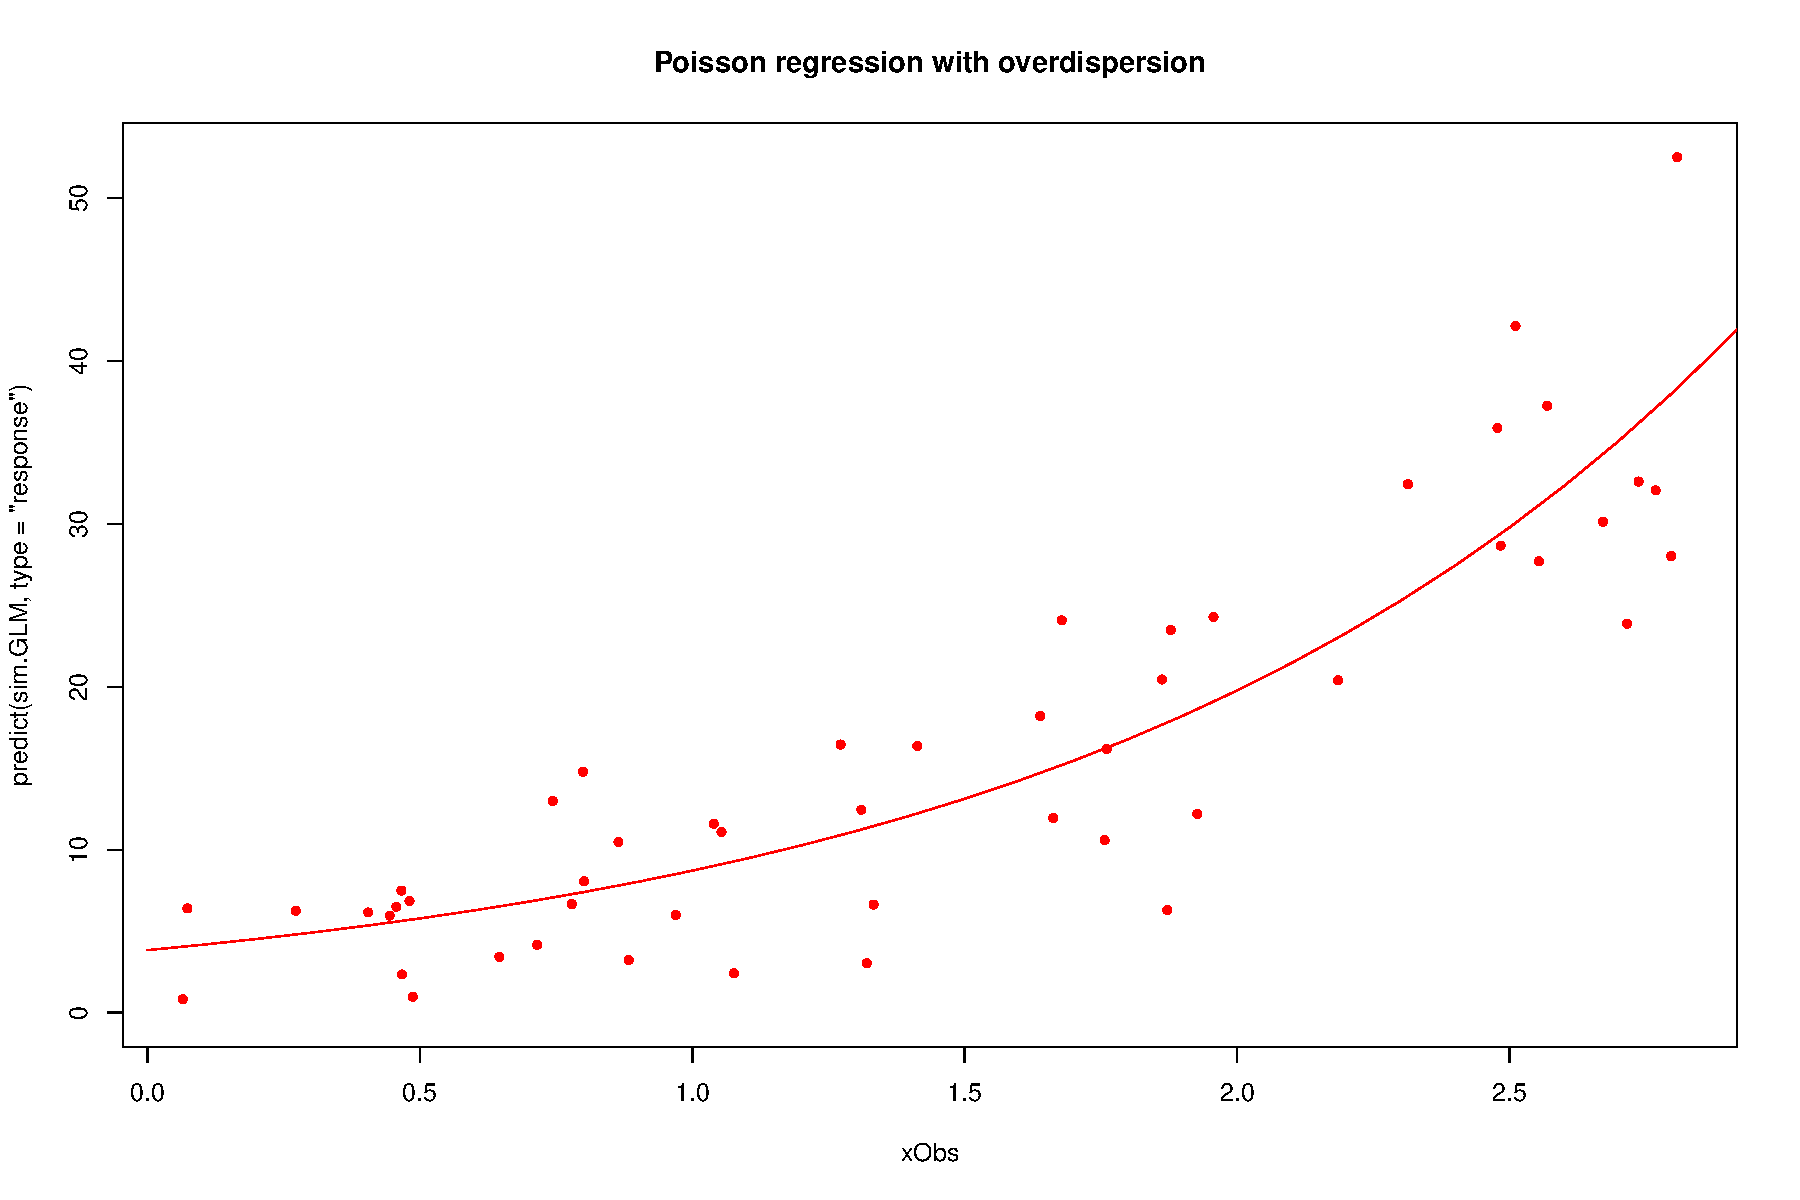
\includegraphics{Lecture06_files/figure-latex/unnamed-chunk-12-1.pdf}

\begin{Shaded}
\begin{Highlighting}[]
\OperatorTok{>}\StringTok{ }\NormalTok{fert.lm <-}\StringTok{ }\KeywordTok{lm}\NormalTok{(TOTFERTRAT}\OperatorTok{~}\NormalTok{ILLITERRAT}\OperatorTok{+}\NormalTok{FEMMARAGE}\OperatorTok{+}\NormalTok{DIVORCERAT}\OperatorTok{+}\NormalTok{TELEPERFAM, }\DataTypeTok{data=}\NormalTok{prov.shp)}
\OperatorTok{>}\StringTok{ }\KeywordTok{summary}\NormalTok{(fert.lm,}\DataTypeTok{corr=}\NormalTok{F)}
\end{Highlighting}
\end{Shaded}

\begin{verbatim}
R> 
R> Call:
R> lm(formula = TOTFERTRAT ~ ILLITERRAT + FEMMARAGE + DIVORCERAT + 
R>     TELEPERFAM, data = prov.shp)
R> 
R> Residuals:
R>      Min       1Q   Median       3Q      Max 
R> -0.21906 -0.06267 -0.00966  0.05425  0.41272 
R> 
R> Coefficients:
R>              Estimate Std. Error t value Pr(>|t|)    
R> (Intercept)  4.496337   0.513726   8.752 1.13e-13 ***
R> ILLITERRAT   0.020377   0.008735   2.333   0.0219 *  
R> FEMMARAGE   -0.088837   0.020771  -4.277 4.71e-05 ***
R> DIVORCERAT  -0.112265   0.055648  -2.017   0.0466 *  
R> TELEPERFAM  -1.226364   0.183037  -6.700 1.76e-09 ***
R> ---
R> Signif. codes:  0 '***' 0.001 '**' 0.01 '*' 0.05 '.' 0.1 ' ' 1
R> 
R> Residual standard error: 0.1035 on 90 degrees of freedom
R> Multiple R-squared:  0.8096, Adjusted R-squared:  0.8012 
R> F-statistic: 95.69 on 4 and 90 DF,  p-value: < 2.2e-16
\end{verbatim}

\begin{Shaded}
\begin{Highlighting}[]
\OperatorTok{>}\StringTok{ }\KeywordTok{vif}\NormalTok{(fert.lm)}
\end{Highlighting}
\end{Shaded}

\begin{verbatim}
R> ILLITERRAT  FEMMARAGE DIVORCERAT TELEPERFAM 
R>   2.601115   2.468365   1.855334   2.088907
\end{verbatim}

\begin{Shaded}
\begin{Highlighting}[]
\OperatorTok{>}\StringTok{ }\CommentTok{# Perform Residual Diagnostics}
\ErrorTok{>}\StringTok{ }\KeywordTok{influenceIndexPlot}\NormalTok{(fert.lm, }\DataTypeTok{id=}\KeywordTok{list}\NormalTok{(}\DataTypeTok{n=}\DecValTok{3}\NormalTok{,}\DataTypeTok{labels=}\NormalTok{prov.shp}\OperatorTok{$}\NormalTok{PROVNAME))}
\end{Highlighting}
\end{Shaded}

\includegraphics{Lecture06_files/figure-latex/unnamed-chunk-12-2.pdf}

\begin{Shaded}
\begin{Highlighting}[]
\OperatorTok{>}\StringTok{ }\NormalTok{fertResid <-}\StringTok{ }\KeywordTok{residuals}\NormalTok{(fert.lm)}
\end{Highlighting}
\end{Shaded}

\hypertarget{identify-potential-outlier}{%
\subsection{Identify potential
outlier}\label{identify-potential-outlier}}

\begin{Shaded}
\begin{Highlighting}[]
\OperatorTok{>}\StringTok{ }\CommentTok{## Why is Bolzano-Bozen an extreme observation? Shall we delete it?}
\ErrorTok{>}\StringTok{ }\NormalTok{idx.max <-}\StringTok{ }\KeywordTok{which.max}\NormalTok{(}\KeywordTok{abs}\NormalTok{(fertResid))        }\CommentTok{# Get index of a record with "outlying" observation }
\OperatorTok{>}\StringTok{ }
\ErrorTok{>}\StringTok{ }\CommentTok{## Map potential outlier}
\ErrorTok{>}\StringTok{ }\NormalTok{extremeObs <-}\StringTok{ }\KeywordTok{rep}\NormalTok{(}\DecValTok{0}\NormalTok{, }\KeywordTok{length}\NormalTok{(fertResid))}
\OperatorTok{>}\StringTok{ }\NormalTok{extremeObs[idx.max] <-}\StringTok{ }\DecValTok{1}
\OperatorTok{>}\StringTok{ }\NormalTok{extremeObs <-}\StringTok{ }\KeywordTok{factor}\NormalTok{(extremeObs, }\DataTypeTok{labels=}\KeywordTok{c}\NormalTok{(}\StringTok{"Population"}\NormalTok{,}\StringTok{"Outlier"}\NormalTok{))}
\OperatorTok{>}\StringTok{ }\KeywordTok{table}\NormalTok{(extremeObs)}
\end{Highlighting}
\end{Shaded}

\begin{verbatim}
R> extremeObs
R> Population    Outlier 
R>         94          1
\end{verbatim}

\begin{Shaded}
\begin{Highlighting}[]
\OperatorTok{>}\StringTok{ }\KeywordTok{plot}\NormalTok{(neig.shp,}\DataTypeTok{axes=}\NormalTok{T,}\DataTypeTok{col=}\KeywordTok{grey}\NormalTok{(}\FloatTok{0.9}\NormalTok{),}\DataTypeTok{border=}\StringTok{"white"}\NormalTok{,                 }\CommentTok{# background: neighboring countries}
\OperatorTok{+}\StringTok{      }\DataTypeTok{xlim=}\NormalTok{prov.bbox[}\DecValTok{1}\NormalTok{,],}\DataTypeTok{ylim=}\NormalTok{prov.bbox[}\DecValTok{2}\NormalTok{,])                     }
\OperatorTok{>}\StringTok{ }\KeywordTok{mapColorQual}\NormalTok{(extremeObs, prov.shp, }\DataTypeTok{map.title=}\StringTok{"Potential Outlier"}\NormalTok{,}
\OperatorTok{+}\StringTok{               }\DataTypeTok{legend.title=}\StringTok{"Outliers"}\NormalTok{, }\DataTypeTok{add.to.map=}\NormalTok{T)        }
\end{Highlighting}
\end{Shaded}

\includegraphics{Lecture06_files/figure-latex/unnamed-chunk-13-1.pdf}

\begin{Shaded}
\begin{Highlighting}[]
\OperatorTok{>}\StringTok{ }\CommentTok{## Inspect outlier}
\ErrorTok{>}\StringTok{ }\NormalTok{prov.shp}\OperatorTok{@}\NormalTok{data[idx.max,]                      }\CommentTok{# List info of record centre is outlier}
\end{Highlighting}
\end{Shaded}

\begin{verbatim}
R>    ID     AREA PROVID  LATCTRD LONGCTRD      PROVNAME REGION RURURB MALEPOP94
R> 49 50 7466.006     21 46698170 11414936 Bolzano-Bozen  North  rural    220787
R>    FEMPOP94 TOTPOP94 POPDENSITY TOTFERTRAT FEMMARAGE DIVORCERAT ILLITERRAT
R> 49   228268   449055   60.14662       1.42     27.88       0.69       0.35
R>    TELEPERFAM
R> 49    0.76808
\end{verbatim}

\begin{Shaded}
\begin{Highlighting}[]
\OperatorTok{>}\StringTok{ }\CommentTok{## Delete outlier or update information}
\ErrorTok{>}\StringTok{ }\CommentTok{#prov.shp <- prov.shp[-idx.max ]             # Delete extreme observation from shapefile }
\ErrorTok{>}\StringTok{ }\NormalTok{prov.shp}\OperatorTok{@}\NormalTok{data[idx.max, }\StringTok{"TOTFERTRAT"}\NormalTok{] <-}\StringTok{ }\FloatTok{1.2}  \CommentTok{# Or change its value within the shapefile}
\OperatorTok{>}\StringTok{ }
\ErrorTok{>}\StringTok{ }\CommentTok{## Continue with updated dataset}
\ErrorTok{>}\StringTok{ }\NormalTok{fert.lm <-}\StringTok{ }\KeywordTok{lm}\NormalTok{(TOTFERTRAT}\OperatorTok{~}\NormalTok{ILLITERRAT}\OperatorTok{+}\NormalTok{FEMMARAGE}\OperatorTok{+}\NormalTok{DIVORCERAT}\OperatorTok{+}\NormalTok{TELEPERFAM,}\DataTypeTok{data=}\NormalTok{prov.shp) }\CommentTok{# update model}
\OperatorTok{>}\StringTok{ }\KeywordTok{summary}\NormalTok{(fert.lm)}
\end{Highlighting}
\end{Shaded}

\begin{verbatim}
R> 
R> Call:
R> lm(formula = TOTFERTRAT ~ ILLITERRAT + FEMMARAGE + DIVORCERAT + 
R>     TELEPERFAM, data = prov.shp)
R> 
R> Residuals:
R>       Min        1Q    Median        3Q       Max 
R> -0.219546 -0.059570 -0.008288  0.055215  0.256479 
R> 
R> Coefficients:
R>              Estimate Std. Error t value Pr(>|t|)    
R> (Intercept)  4.625004   0.476205   9.712 1.13e-15 ***
R> ILLITERRAT   0.021280   0.008097   2.628   0.0101 *  
R> FEMMARAGE   -0.095354   0.019254  -4.953 3.41e-06 ***
R> DIVORCERAT  -0.111163   0.051584  -2.155   0.0338 *  
R> TELEPERFAM  -1.173424   0.169668  -6.916 6.54e-10 ***
R> ---
R> Signif. codes:  0 '***' 0.001 '**' 0.01 '*' 0.05 '.' 0.1 ' ' 1
R> 
R> Residual standard error: 0.09594 on 90 degrees of freedom
R> Multiple R-squared:  0.8345, Adjusted R-squared:  0.8272 
R> F-statistic: 113.5 on 4 and 90 DF,  p-value: < 2.2e-16
\end{verbatim}

\begin{Shaded}
\begin{Highlighting}[]
\OperatorTok{>}\StringTok{ }\KeywordTok{influenceIndexPlot}\NormalTok{(fert.lm, }\DataTypeTok{id=}\KeywordTok{list}\NormalTok{(}\DataTypeTok{n=}\DecValTok{3}\NormalTok{, }\DataTypeTok{labels=}\NormalTok{prov.shp}\OperatorTok{$}\NormalTok{PROVNAME))}
\end{Highlighting}
\end{Shaded}

\includegraphics{Lecture06_files/figure-latex/unnamed-chunk-13-2.pdf}

\hypertarget{check-for-heteroscedasticity}{%
\subsection{Check for
heteroscedasticity}\label{check-for-heteroscedasticity}}

\begin{Shaded}
\begin{Highlighting}[]
\OperatorTok{>}\StringTok{ }\CommentTok{## Check for heteroscedasticity}
\ErrorTok{>}\StringTok{ }\NormalTok{fert.fgls <-}\StringTok{ }\KeywordTok{lmHetero}\NormalTok{(TOTFERTRAT}\OperatorTok{~}\NormalTok{ILLITERRAT}\OperatorTok{+}\NormalTok{FEMMARAGE}\OperatorTok{+}\NormalTok{DIVORCERAT}\OperatorTok{+}\NormalTok{TELEPERFAM }\OperatorTok{|}\StringTok{ }\KeywordTok{log}\NormalTok{(FEMPOP94),}
\OperatorTok{+}\StringTok{                       }\DataTypeTok{data=}\NormalTok{prov.shp)}
\OperatorTok{>}\StringTok{ }\KeywordTok{summary}\NormalTok{(fert.fgls)}
\end{Highlighting}
\end{Shaded}

\begin{verbatim}
R> 
R> ================================================================
R> Multiplicatively Weighted Heteroscedasticity ML-Regression Model
R> ================================================================
R> 
R> Call:
R> lmHetero(formula = TOTFERTRAT ~ ILLITERRAT + FEMMARAGE + DIVORCERAT + 
R>     TELEPERFAM | log(FEMPOP94), data = prov.shp)
R> 
R> Regression Coefficients:
R>               Estimate    Std.Err z-value  Pr(>|z|)    
R> (Intercept)  4.3881835  0.4265870 10.2867 < 2.2e-16 ***
R> ILLITERRAT   0.0286213  0.0074558  3.8388 0.0001236 ***
R> FEMMARAGE   -0.0894065  0.0174198 -5.1325 2.860e-07 ***
R> DIVORCERAT  -0.1073668  0.0441414 -2.4323 0.0150017 *  
R> TELEPERFAM  -1.1055990  0.1775114 -6.2283 4.714e-10 ***
R> ---
R> Signif. codes:  0 '***' 0.001 '**' 0.01 '*' 0.05 '.' 0.1 ' ' 1
R> 
R> Gamma Coefficients:
R>                   Gamma   Std.Err z-value  Pr(>|z|)    
R> (Intercept)   -12.60936   2.56690 -4.9123 9.001e-07 ***
R> log(FEMPOP94)   0.63263   0.20748  3.0492  0.002295 ** 
R> ---
R> Signif. codes:  0 '***' 0.001 '**' 0.01 '*' 0.05 '.' 0.1 ' ' 1
R> 
R> log-likelihood = 92.96326 
R> 
R> Heteroscedasticity likelihood ratio test:
R>        LR   df  Pr(Chi > LR)
R>  5.019431    1    0.02506441
\end{verbatim}

Note the possitive sign of \(\gamma_2\) is contradicting theory. This is
marginal significant of the heteroscedastic model and will be used
subsequently for demonstration purposes.

Therefore, the lm-model is updated to a weighted lm-model.

\begin{Shaded}
\begin{Highlighting}[]
\OperatorTok{>}\StringTok{ }\NormalTok{fert.wlm <-}\StringTok{ }\KeywordTok{lm}\NormalTok{(TOTFERTRAT}\OperatorTok{~}\NormalTok{ILLITERRAT}\OperatorTok{+}\NormalTok{FEMMARAGE}\OperatorTok{+}\NormalTok{DIVORCERAT}\OperatorTok{+}\NormalTok{TELEPERFAM, }\DataTypeTok{data=}\NormalTok{prov.shp,}
\OperatorTok{+}\StringTok{                }\DataTypeTok{weights=}\NormalTok{fert.fgls}\OperatorTok{$}\NormalTok{weights)}
\OperatorTok{>}\StringTok{ }\KeywordTok{summary}\NormalTok{(fert.wlm)}
\end{Highlighting}
\end{Shaded}

\begin{verbatim}
R> 
R> Call:
R> lm(formula = TOTFERTRAT ~ ILLITERRAT + FEMMARAGE + DIVORCERAT + 
R>     TELEPERFAM, data = prov.shp, weights = fert.fgls$weights)
R> 
R> Weighted Residuals:
R>      Min       1Q   Median       3Q      Max 
R> -2.51018 -0.61717  0.02056  0.60411  2.81691 
R> 
R> Coefficients:
R>             Estimate Std. Error t value Pr(>|t|)    
R> (Intercept)  4.38815    0.43827  10.012 2.69e-16 ***
R> ILLITERRAT   0.02862    0.00766   3.737 0.000327 ***
R> FEMMARAGE   -0.08941    0.01790  -4.996 2.86e-06 ***
R> DIVORCERAT  -0.10737    0.04535  -2.367 0.020052 *  
R> TELEPERFAM  -1.10560    0.18238  -6.062 3.09e-08 ***
R> ---
R> Signif. codes:  0 '***' 0.001 '**' 0.01 '*' 0.05 '.' 0.1 ' ' 1
R> 
R> Residual standard error: 1.027 on 90 degrees of freedom
R> Multiple R-squared:  0.8419, Adjusted R-squared:  0.8348 
R> F-statistic: 119.8 on 4 and 90 DF,  p-value: < 2.2e-16
\end{verbatim}

\hypertarget{map-the-regression-residual}{%
\subsection{Map the regression
residual}\label{map-the-regression-residual}}

\begin{Shaded}
\begin{Highlighting}[]
\OperatorTok{>}\StringTok{ }\CommentTok{## Plot Regression Residuals (Bi-polar)}
\ErrorTok{>}\StringTok{ }\NormalTok{fertResid <-}\StringTok{ }\KeywordTok{weighted.residuals}\NormalTok{(fert.wlm)                }\CommentTok{# Update residuals}
\OperatorTok{>}\StringTok{ }\KeywordTok{hist}\NormalTok{(fertResid, }\DataTypeTok{main=}\StringTok{"Residuals of Weighted Model"}\NormalTok{)      }\CommentTok{# Explore distribution to}
\end{Highlighting}
\end{Shaded}

\includegraphics{Lecture06_files/figure-latex/residmap-1.pdf}

\begin{Shaded}
\begin{Highlighting}[]
\OperatorTok{>}\StringTok{ }\KeywordTok{length}\NormalTok{(fertResid[fertResid }\OperatorTok{<}\StringTok{ }\DecValTok{0}\NormalTok{])                         }\CommentTok{# identify number of pos/neg classes}
\end{Highlighting}
\end{Shaded}

\begin{verbatim}
R> [1] 46
\end{verbatim}

\begin{Shaded}
\begin{Highlighting}[]
\OperatorTok{>}\StringTok{ }\KeywordTok{length}\NormalTok{(fertResid[fertResid }\OperatorTok{>=}\StringTok{ }\DecValTok{0}\NormalTok{])}
\end{Highlighting}
\end{Shaded}

\begin{verbatim}
R> [1] 49
\end{verbatim}

\begin{Shaded}
\begin{Highlighting}[]
\OperatorTok{>}\StringTok{ }\KeywordTok{plot}\NormalTok{(neig.shp,}\DataTypeTok{axes=}\NormalTok{T,}\DataTypeTok{col=}\KeywordTok{grey}\NormalTok{(}\FloatTok{0.9}\NormalTok{),}\DataTypeTok{border=}\StringTok{"white"}\NormalTok{,}
\OperatorTok{+}\StringTok{      }\DataTypeTok{xlim=}\NormalTok{prov.bbox[}\DecValTok{1}\NormalTok{,],}\DataTypeTok{ylim=}\NormalTok{prov.bbox[}\DecValTok{2}\NormalTok{,])               }\CommentTok{# first background}
\OperatorTok{>}\StringTok{ }\KeywordTok{mapBiPolar}\NormalTok{(fertResid, prov.shp,                           }\CommentTok{# second regression residuals}
\OperatorTok{+}\StringTok{             }\DataTypeTok{neg.breaks=}\DecValTok{5}\NormalTok{, }\DataTypeTok{pos.breaks=}\DecValTok{4}\NormalTok{, }\DataTypeTok{break.value=}\FloatTok{0.0}\NormalTok{, }
\OperatorTok{+}\StringTok{             }\DataTypeTok{map.title=}\StringTok{"Fertility Model Residuals"}\NormalTok{,}
\OperatorTok{+}\StringTok{             }\DataTypeTok{legend.title=}\StringTok{"Residuals"}\NormalTok{, }
\OperatorTok{+}\StringTok{             }\DataTypeTok{legend.cex=}\FloatTok{1.7}\NormalTok{, }\DataTypeTok{add.to.map=}\NormalTok{T)}
\end{Highlighting}
\end{Shaded}

\includegraphics{Lecture06_files/figure-latex/residmap-2.pdf}

The map pattern indicates that there are spatial clusters with positive
and negative regression residuals. Thus the independence assumption is
violated.

\hypertarget{identify-the-linkage-structure}{%
\subsection{Identify the linkage
structure}\label{identify-the-linkage-structure}}

\begin{Shaded}
\begin{Highlighting}[]
\OperatorTok{>}\StringTok{ }\CommentTok{## Plot Augmented Spatial Links among Italian Provinces}
\ErrorTok{>}\StringTok{ }\CommentTok{## Notes: Shape file has been edited so satellite islands are connected to mainland}
\ErrorTok{>}\StringTok{ }\CommentTok{## Alternatively spdep::edit.nb function (does not work with RStudio)}
\ErrorTok{>}\StringTok{ }\NormalTok{prov.link <-}\StringTok{ }\KeywordTok{poly2nb}\NormalTok{(prov.shp, }\DataTypeTok{queen=}\NormalTok{F)                          }\CommentTok{# Generate neighbors links}
\OperatorTok{>}\StringTok{ }
\ErrorTok{>}\StringTok{ }\KeywordTok{plot}\NormalTok{(neig.shp,}\DataTypeTok{axes=}\NormalTok{T,}\DataTypeTok{col=}\KeywordTok{grey}\NormalTok{(}\FloatTok{0.9}\NormalTok{),}\DataTypeTok{border=}\StringTok{"white"}\NormalTok{,}
\OperatorTok{+}\StringTok{      }\DataTypeTok{xlim=}\NormalTok{prov.bbox[}\DecValTok{1}\NormalTok{,],}\DataTypeTok{ylim=}\NormalTok{prov.bbox[}\DecValTok{2}\NormalTok{,])                      }\CommentTok{# First background}
\OperatorTok{>}\StringTok{ }\KeywordTok{plot}\NormalTok{(prov.shp,}\DataTypeTok{col=}\StringTok{"palegreen3"}\NormalTok{ ,}\DataTypeTok{border=}\KeywordTok{grey}\NormalTok{(}\FloatTok{0.9}\NormalTok{), }\DataTypeTok{axes=}\NormalTok{T, }\DataTypeTok{add=}\NormalTok{T) }\CommentTok{# Second plot areas}
\OperatorTok{>}\StringTok{ }\KeywordTok{plot}\NormalTok{(prov.link,}\DataTypeTok{coords=}\NormalTok{prov.centroid, }\DataTypeTok{pch=}\DecValTok{19}\NormalTok{, }\DataTypeTok{cex=}\FloatTok{0.1}\NormalTok{,            }\CommentTok{# Third plot links focused at centroids}
\OperatorTok{+}\StringTok{      }\DataTypeTok{col=}\StringTok{"blue"}\NormalTok{, }\DataTypeTok{add=}\NormalTok{T)}
\OperatorTok{>}\StringTok{ }\KeywordTok{title}\NormalTok{(}\StringTok{"Augmented Spatial Links among Provinces"}\NormalTok{)                 }\CommentTok{# Forth add title}
\OperatorTok{>}\StringTok{ }\KeywordTok{box}\NormalTok{()                                                            }\CommentTok{# Fifth refresh frame}
\end{Highlighting}
\end{Shaded}

\includegraphics{Lecture06_files/figure-latex/linkmap-1.pdf}

\hypertarget{perform-a-test-for-spatial-autocorrelation-in-the-residuals}{%
\subsection{Perform a test for spatial autocorrelation in the
residuals}\label{perform-a-test-for-spatial-autocorrelation-in-the-residuals}}

\begin{Shaded}
\begin{Highlighting}[]
\OperatorTok{>}\StringTok{ }\NormalTok{prov.linkW <-}\StringTok{ }\KeywordTok{nb2listw}\NormalTok{(prov.link, }\DataTypeTok{style=}\StringTok{"W"}\NormalTok{)                   }\CommentTok{# generated row-sum standardized neighbors list}
\OperatorTok{>}\StringTok{ }\NormalTok{spOutliers <-}\StringTok{ }\KeywordTok{moran.plot}\NormalTok{(}\KeywordTok{weighted.residuals}\NormalTok{(fert.wlm),         }\CommentTok{# Moran plot with outlier diagnositics}
\OperatorTok{+}\StringTok{                          }\NormalTok{prov.linkW, }\DataTypeTok{labels=}\NormalTok{prov.shp}\OperatorTok{$}\NormalTok{PROVNAME)          }
\end{Highlighting}
\end{Shaded}

\includegraphics{Lecture06_files/figure-latex/morantest-1.pdf}

\begin{Shaded}
\begin{Highlighting}[]
\OperatorTok{>}\StringTok{ }\KeywordTok{lm.morantest}\NormalTok{(fert.wlm, prov.linkW)                             }\CommentTok{# Test with W-coding scheme}
\end{Highlighting}
\end{Shaded}

\begin{verbatim}
R> 
R>  Global Moran I for regression residuals
R> 
R> data:  
R> model: lm(formula = TOTFERTRAT ~ ILLITERRAT + FEMMARAGE + DIVORCERAT +
R> TELEPERFAM, data = prov.shp, weights = fert.fgls$weights)
R> weights: prov.linkW
R> 
R> Moran I statistic standard deviate = 4.5306, p-value = 2.941e-06
R> alternative hypothesis: greater
R> sample estimates:
R> Observed Moran I      Expectation         Variance 
R>      0.281242173     -0.029598120      0.004707174
\end{verbatim}

Also look up \texttt{help(lm.morantest)}. Internally weighted regression
residuals are used.

\hypertarget{maximum-likelihood-estimation-of-sar}{%
\subsection{Maximum likelihood estimation of
SAR}\label{maximum-likelihood-estimation-of-sar}}

Check the online help for the \texttt{spdep::spautolm(\ )} function.
Note the use of the \texttt{weights} option here. When the
\texttt{weights} option is used \texttt{spautolm} requires a full
specification of the model rather than just using the \texttt{fert.wlm}
object.

\begin{Shaded}
\begin{Highlighting}[]
\OperatorTok{>}\StringTok{ }\NormalTok{fert.SAR <-}\StringTok{ }\KeywordTok{spautolm}\NormalTok{(TOTFERTRAT}\OperatorTok{~}\NormalTok{ILLITERRAT}\OperatorTok{+}\NormalTok{FEMMARAGE}\OperatorTok{+}\NormalTok{DIVORCERAT}\OperatorTok{+}\NormalTok{TELEPERFAM, }
\OperatorTok{+}\StringTok{                      }\DataTypeTok{data=}\NormalTok{prov.shp, }\DataTypeTok{weights =}\NormalTok{ fert.fgls}\OperatorTok{$}\NormalTok{weights,}
\OperatorTok{+}\StringTok{                      }\DataTypeTok{na.action=}\StringTok{"na.omit"}\NormalTok{, }\DataTypeTok{listw=}\NormalTok{prov.linkW, }\DataTypeTok{family=}\StringTok{"SAR"}\NormalTok{)}
\OperatorTok{>}\StringTok{ }\KeywordTok{summary}\NormalTok{(fert.SAR)}
\end{Highlighting}
\end{Shaded}

\begin{verbatim}
R> 
R> Call: spautolm(formula = TOTFERTRAT ~ ILLITERRAT + FEMMARAGE + DIVORCERAT + 
R>     TELEPERFAM, data = prov.shp, listw = prov.linkW, weights = fert.fgls$weights, 
R>     na.action = "na.omit", family = "SAR")
R> 
R> Residuals:
R>        Min         1Q     Median         3Q        Max 
R> -0.1346010 -0.0515529  0.0066078  0.0595509  0.2377229 
R> 
R> Coefficients: 
R>               Estimate Std. Error z value  Pr(>|z|)
R> (Intercept)  3.1164030  0.4694416  6.6385 3.168e-11
R> ILLITERRAT   0.0166445  0.0089083  1.8684  0.061701
R> FEMMARAGE   -0.0484661  0.0178010 -2.7227  0.006476
R> DIVORCERAT  -0.0309038  0.0378188 -0.8172  0.413840
R> TELEPERFAM  -0.9134920  0.1668045 -5.4764 4.340e-08
R> 
R> Lambda: 0.76152 LR test value: 23.96 p-value: 9.8382e-07 
R> Numerical Hessian standard error of lambda: 0.092528 
R> 
R> Log likelihood: 104.943 
R> ML residual variance (sigma squared): 0.63854, (sigma: 0.79909)
R> Number of observations: 95 
R> Number of parameters estimated: 7 
R> AIC: -195.89
\end{verbatim}

The likelihood ratio test of the SAR model is identically to the hand
calculated one. Important here is a slight difference in the calculation
when heteroscedasticity is incorporated.

\begin{Shaded}
\begin{Highlighting}[]
\OperatorTok{>}\StringTok{ }\CommentTok{## Likelihood Ratio test (identical to LR from spautolm)}
\ErrorTok{>}\StringTok{ }\CommentTok{#(likeH0 <- logLik(fert.lm))                     # Use for unweighted model}
\ErrorTok{>}\StringTok{ }\NormalTok{likeH0 <-}\StringTok{ }\NormalTok{fert.fgls}\OperatorTok{$}\NormalTok{logLikeH1}
\OperatorTok{>}\StringTok{ }\NormalTok{(likeH1 <-}\StringTok{ }\KeywordTok{logLik}\NormalTok{(fert.SAR))}
\end{Highlighting}
\end{Shaded}

\begin{verbatim}
R> Warning: Method logLik.spautolm moved to the spatialreg package
\end{verbatim}

\begin{verbatim}
R> Warning in logLik.spautolm(fert.SAR): install the spatialreg package
\end{verbatim}

\begin{verbatim}
R> 'log Lik.' 104.943 (df=7)
\end{verbatim}

\begin{Shaded}
\begin{Highlighting}[]
\OperatorTok{>}\StringTok{ }\KeywordTok{cat}\NormalTok{(}\StringTok{"chi-square value:  "}\NormalTok{, chi <-}\StringTok{ }\DecValTok{-2}\OperatorTok{*}\NormalTok{(likeH0[}\DecValTok{1}\NormalTok{]}\OperatorTok{-}\NormalTok{likeH1[}\DecValTok{1}\NormalTok{]))}
\end{Highlighting}
\end{Shaded}

\begin{verbatim}
R> chi-square value:   23.95954
\end{verbatim}

\begin{Shaded}
\begin{Highlighting}[]
\OperatorTok{>}\StringTok{ }\KeywordTok{cat}\NormalTok{(}\StringTok{"}\CharTok{\textbackslash{}n}\StringTok{error-probability: "}\NormalTok{, }\KeywordTok{pchisq}\NormalTok{(chi, }\DataTypeTok{df=}\DecValTok{1}\NormalTok{, }\DataTypeTok{lower.tail=}\NormalTok{F))}
\end{Highlighting}
\end{Shaded}

\begin{verbatim}
R> 
R> error-probability:  9.838169e-07
\end{verbatim}

Check whether the residuals are as expected free of spatial
autocorrelation. Because the distribution of ML residuals in unknown,
Morans's \(I\) is evaluated here using a randomization approach.

\begin{Shaded}
\begin{Highlighting}[]
\OperatorTok{>}\StringTok{ }\CommentTok{## Moran test applying randomization because ML may not be normal distributed}
\ErrorTok{>}\StringTok{ }\KeywordTok{plot}\NormalTok{(neig.shp,}\DataTypeTok{axes=}\NormalTok{T,}\DataTypeTok{col=}\KeywordTok{grey}\NormalTok{(}\FloatTok{0.9}\NormalTok{),}\DataTypeTok{border=}\StringTok{"white"}\NormalTok{,}
\OperatorTok{+}\StringTok{      }\DataTypeTok{xlim=}\NormalTok{prov.bbox[}\DecValTok{1}\NormalTok{,],}\DataTypeTok{ylim=}\NormalTok{prov.bbox[}\DecValTok{2}\NormalTok{,])                        }\CommentTok{# first background}
\OperatorTok{>}\StringTok{ }\KeywordTok{mapBiPolar}\NormalTok{(}\KeywordTok{residuals}\NormalTok{(fert.SAR), prov.shp,                          }\CommentTok{# second regression residuals}
\OperatorTok{+}\StringTok{             }\DataTypeTok{neg.breaks=}\DecValTok{5}\NormalTok{, }\DataTypeTok{pos.breaks=}\DecValTok{4}\NormalTok{, }\DataTypeTok{break.value=}\FloatTok{0.0}\NormalTok{, }
\OperatorTok{+}\StringTok{             }\DataTypeTok{map.title=}\StringTok{"Fertility SAR Model Residuals"}\NormalTok{,}
\OperatorTok{+}\StringTok{             }\DataTypeTok{legend.title=}\StringTok{"Residuals"}\NormalTok{, }\DataTypeTok{legend.cex =} \FloatTok{1.6}\NormalTok{,}
\OperatorTok{+}\StringTok{             }\DataTypeTok{add.to.map=}\NormalTok{T)}
\end{Highlighting}
\end{Shaded}

\begin{verbatim}
R> Warning: Method residuals.spautolm moved to the spatialreg package
\end{verbatim}

\begin{verbatim}
R> Warning in residuals.spautolm(fert.SAR): install the spatialreg package
\end{verbatim}

\includegraphics{Lecture06_files/figure-latex/SARresid-1.pdf}

\begin{Shaded}
\begin{Highlighting}[]
\OperatorTok{>}\StringTok{ }\CommentTok{## Evaluate ML residuals for spatial autocorrelation}
\ErrorTok{>}\StringTok{ }\KeywordTok{moran.mc}\NormalTok{(}\KeywordTok{residuals}\NormalTok{(fert.SAR), prov.linkW, }\DataTypeTok{nsim=}\DecValTok{9999}\NormalTok{) }
\end{Highlighting}
\end{Shaded}

\begin{verbatim}
R> Warning: Method residuals.spautolm moved to the spatialreg package

R> Warning: install the spatialreg package
\end{verbatim}

\begin{verbatim}
R> 
R>  Monte-Carlo simulation of Moran I
R> 
R> data:  residuals(fert.SAR) 
R> weights: prov.linkW  
R> number of simulations + 1: 10000 
R> 
R> statistic = -0.060189, observed rank = 2455, p-value = 0.7545
R> alternative hypothesis: greater
\end{verbatim}

\end{document}
